%!TEX root = paper.tex
%%%%%%%%%%%%%%%%%%%%%%%%%%%%%%%%%%%%%%%%%%%%%%%%%%%%%%%%%%%%%%%%%%%%%%%%%%%%%%%%
\section{An End-to-End Lag Model}
\label{sec:model}

\begin{figure}[!t]
	\centering
	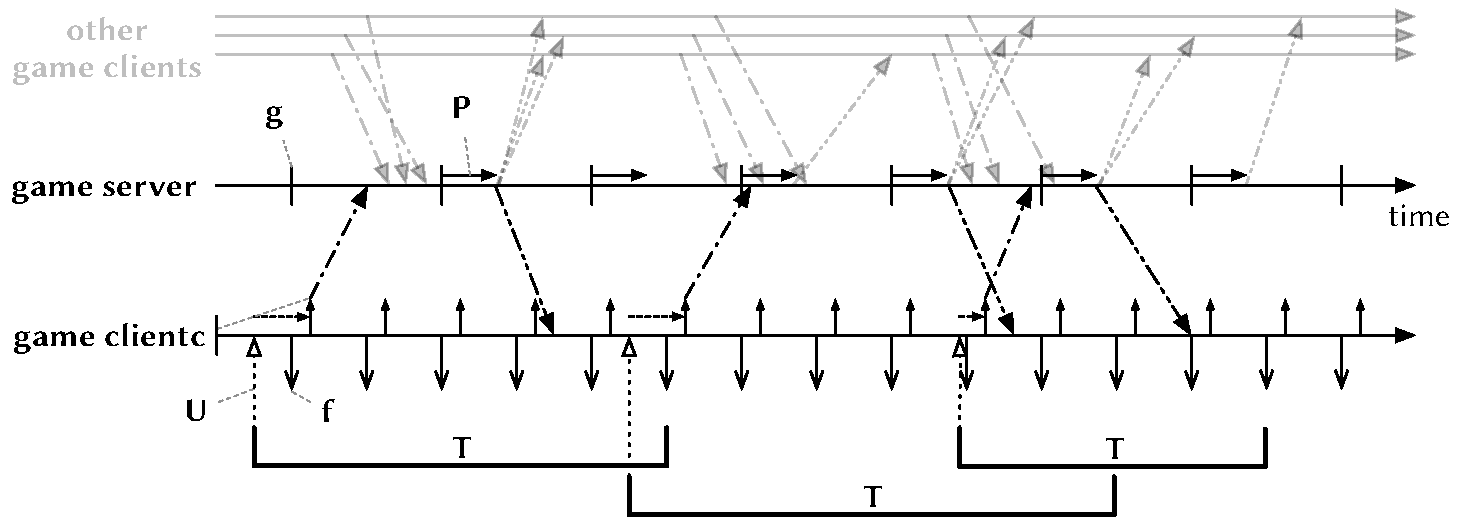
\includegraphics[width=1.0\columnwidth]{../../models/tickrate-timeseries-notation.pdf}
	\caption{Exemplary flow of events in an online client-server game, and resulting end-to-end lag.
	}
\label{fig:tickrate-timeseries}
\end{figure}

To combat some of these open issues, a simplified end-to-end model and simulation was set up to investigate lag in both offline and online games and its relationship with the framerate and tickrate. Fig.~\ref{fig:tickrate-timeseries} shows the flow of events between game client and server for the simplified case of an online video game. % This is further discussed in our publication in [PQS?]
Based on the model a simulator\footnote{\url{https://github.com/mas-ude/onlinegame-lag-sim/tree/master/simulation}} was created.

\begin{figure}[!t]
	\centering
	\vspace{-6mm}
	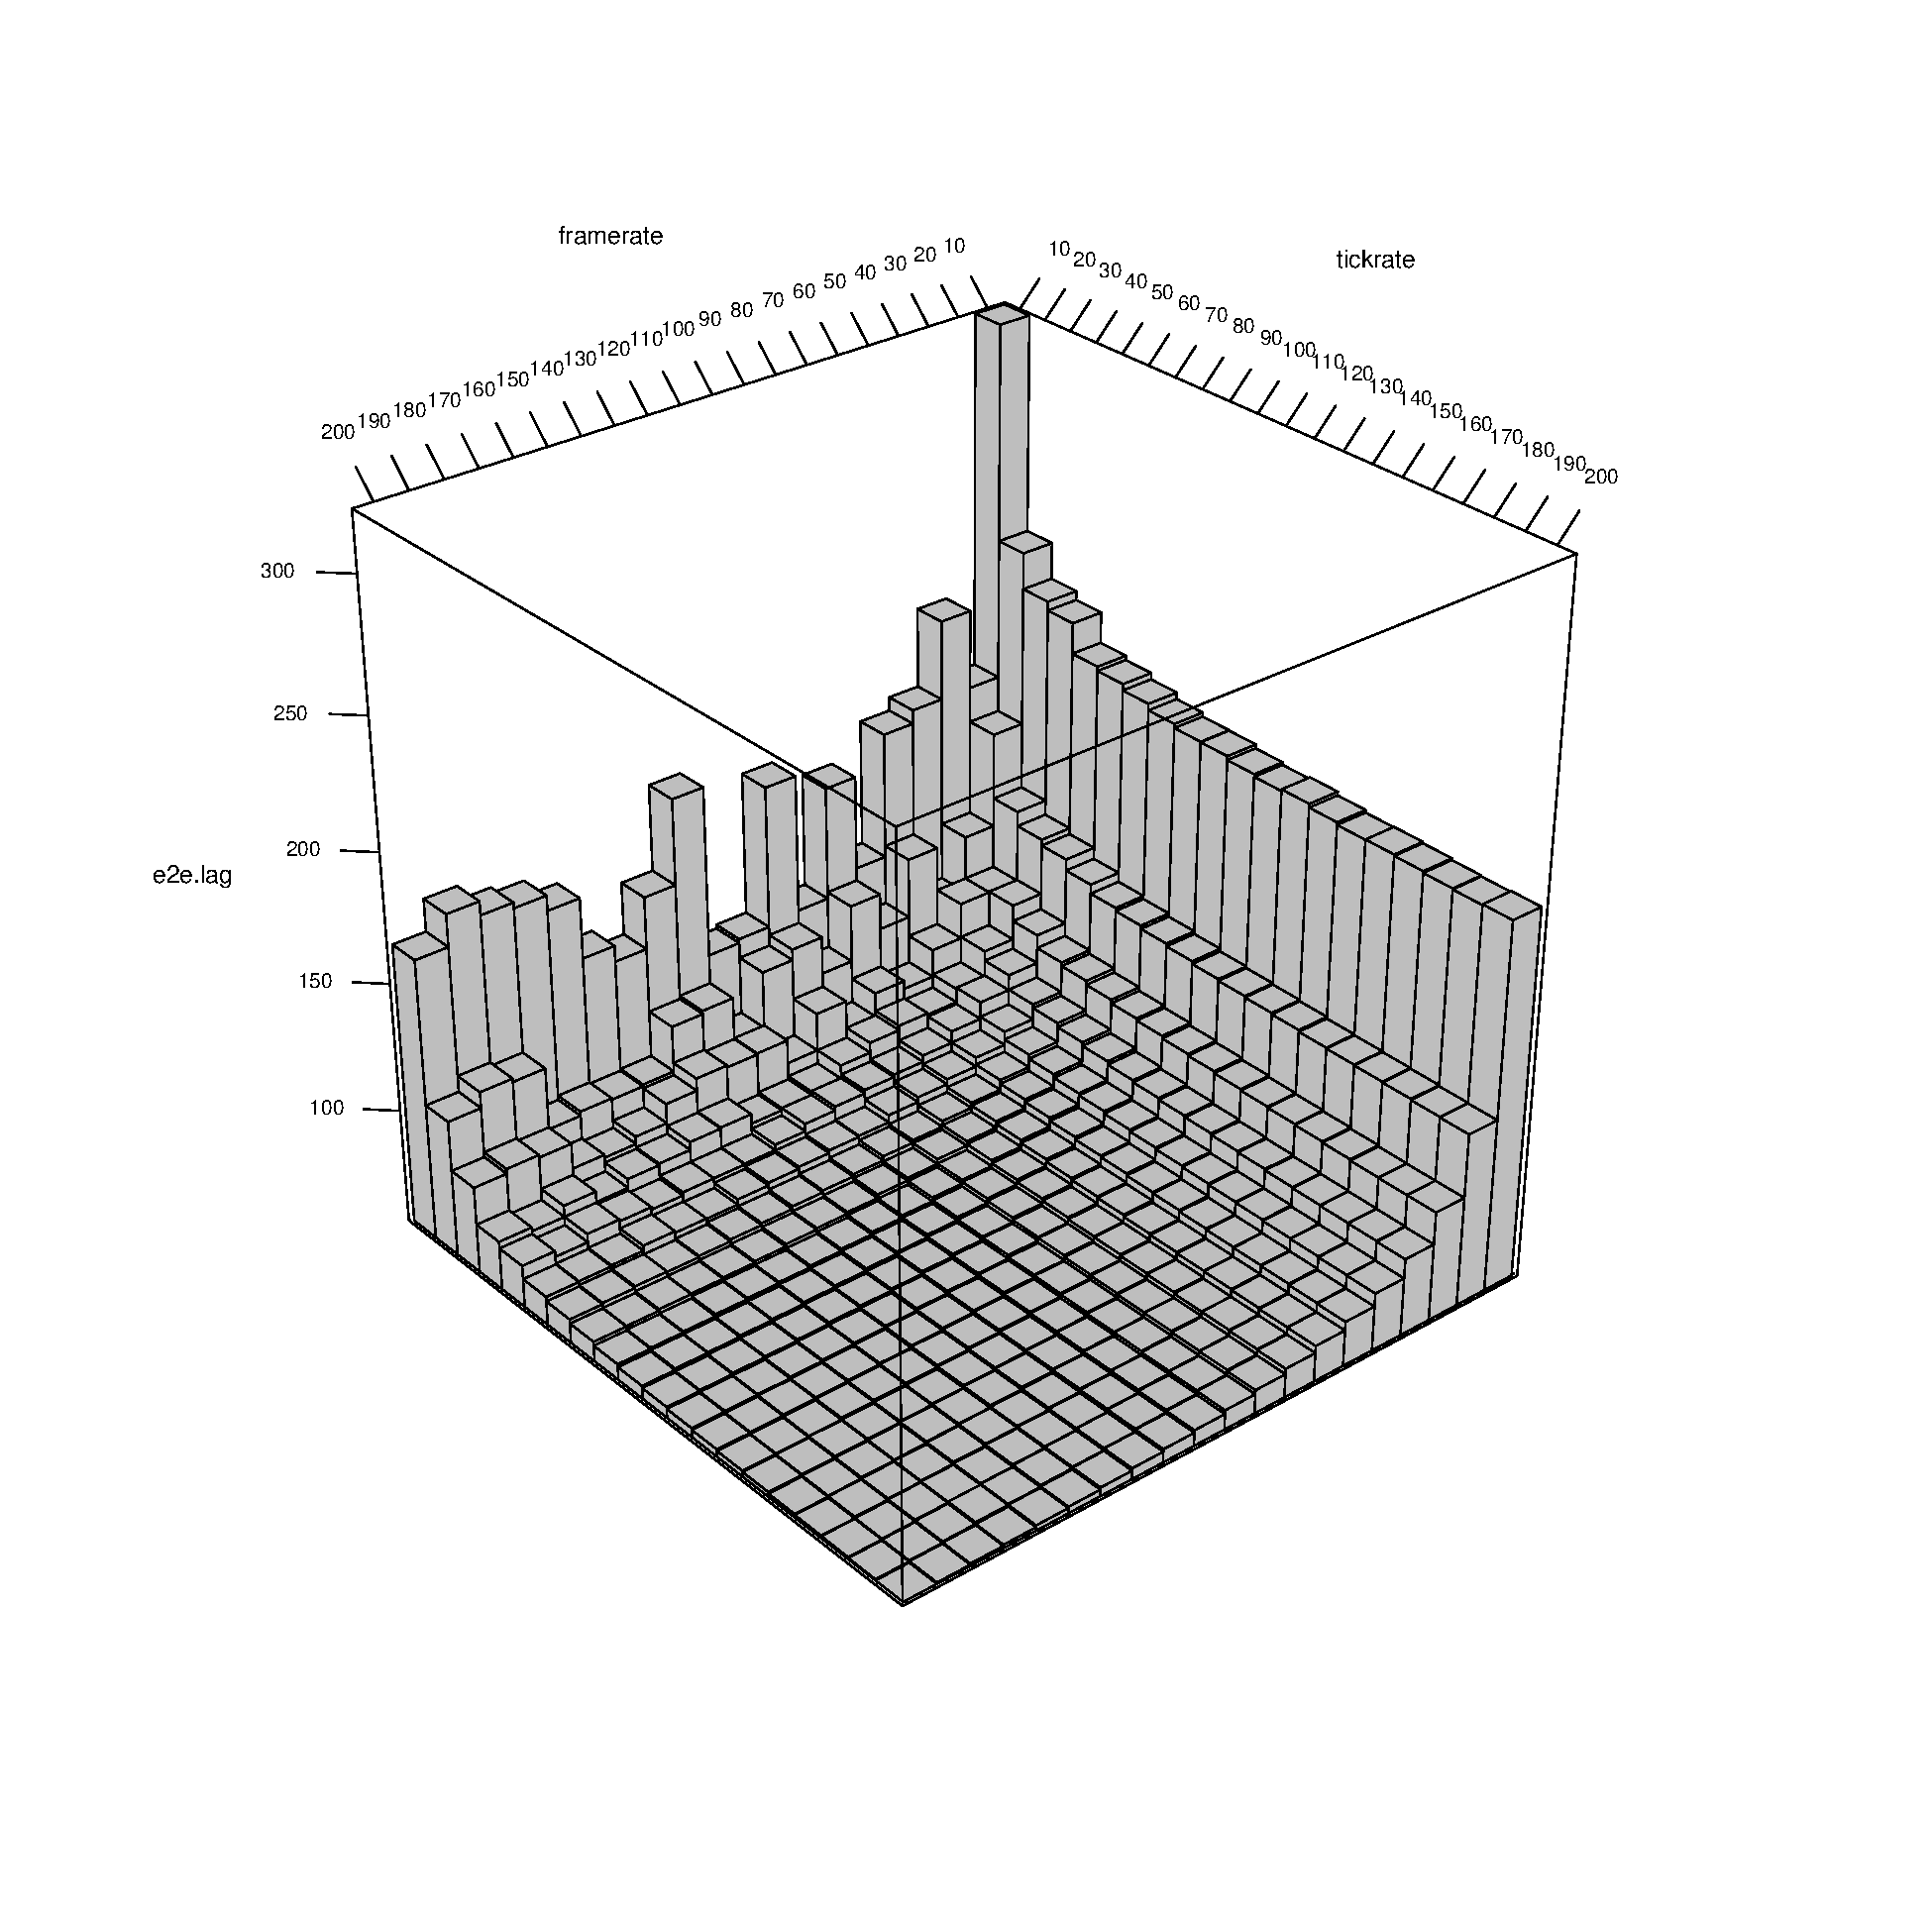
\includegraphics[width=1.0\columnwidth]{../../simulation/visualization/e2e-lag-3dbars.pdf}
	\vspace{-15mm}
	\caption{Influence of client framerate and server tickrate on the median end-to-end lag in the online game scenario.}
\label{fig:3dbars-framerate-tickrate-lag}
\end{figure}

Consider the scenario of an online video game as depicted in Fig.~\ref{fig:3dbars-framerate-tickrate-lag}, with network lag and server processing time included. The framerate has a larger influence on the lag than the tickrate. Second, for low framerates and tickrates, the impact of network delay on the end-to-end lag is almost completely masked. Only if both rates are high enough, the network delay will play a more significant role. This masking effect has large implications for video games and their evaluation. Many evaluations examine the influence of the network delay only, without considering other contributions to end-to-end lag. These results indicate that this might not be the best course of action. Another noteworthy result is the much larger variance of lag in the framerate dimension when compared to the tickrate. This requires video game studies to have a very high repetition rate to provide meaningful results. Furthermore, this also implies the neccessity of a tight control over game parameters, such as the framerate, resolution, or input devices, in accordance with the game's type. In order to properly determine this type, novel ways to classify games are needed, as games from the same genre can be vastly different in terms of game speed and necessary reaction times.

% \subsection{Model Simplifications}

% These simulation models do not attempt to capture all possible sources of lag that. Indeed, we simplify the models in the following aspects in the hope to make the results more tractable.
% %\textbf{TODO Make this more of a ``future work'' section, less ``why we suck''.}

% \subsubsection{Additional delay sources}
% The models ignore the delays contributed by input devices like keyboards, mice, and game controllers. We estimate these at below \SI{10}{\milli\second}. The same goes for the lag of the display device (from after rendering or decoding until the frame is actually visible) which is typically in the range of 1--3 frame times for a computer monitor, and larger for TV sets. The models can be extended to take those delay factors into account, but they were exempted for the sake of simplicity in this paper.
% % TODO: \textbf{Add adaptive VSYNC?}

% \subsubsection{Subtleties of game internals}
% Modern games go great lengths to handle lag gracefully, and try to ``work around it'' in various ways. The methods for this vary, and implementations usually are not open for examination, so we leave them for further study. Techniques include lag compensation (the game client tries to predict the server state from past knowledge, allowing for smoother local updates but possibly causing slight deviation and re-synchronization artifacts), and tick- and framerate adaptation at the game server and client, respectively. Lastly, player actions in a game might take multiple command time intervals to perform. The simulation currently assumes that every single batch of commands that reaches the server will result in state updates and thus changes in the perceptible output of the game client. It should be noted that none of these techniques alter the end-to-end lag itself, rather they just try to conceal it on some higher level. Therefore, the mechanisms do not invalidate our examination.

% \subsubsection{Factors in human perception and strategy}
% The models we present do not take into account the perceived lag from when the players \textit{think} they have triggered an action to when they perceive the outcomes of their action. This consequently disregards effects of different player actions, strategies, and so on.







%%%%%%%%%%%%%%%%%%%%%%%%%%%%%%%%%%%%%%%%%%%%%%%%%%%%%%%%%%%%%%%%%%%%%%%%%%%%%%%%
% \subsubsection{Local Games}

% The first and simplest scenario to be investigated here is the case of the local game. In the version implemented here, the tickrate is still present, but the influence of the network is entirely removed. It therefore represents the best case an online multiplayer game could achieve if the server ran locally.

% The values can be estimated as follows. Every user input event traverses three queues with fixed-rate outputs ($c=g$, g, and $f$), and every game state update waits for the next full frame until it gets displayed. In the ideal case, an input event occurs just before the command message is sent off, the server tick follows as soon as the message is received, and the update reaches the client just before a frame is output. Then the end-to-end lag is slightly above the frame time that must elapse before the update can be rendered to screen, $T_{min}>f^{-1}$.

% In case the events are unfavorably offset against one another, an input event has to wait almost a full command-message cycle until it is sent on; it reaches the server just after a tick has occurred, so it waits almost a full server tick; finally, it will wait for almost two frame times until it is displayed. Combining with the previous result bounds the lag as follows, $f^{-1} < T < c^{-1}+g^{-1}+2f^{-1}$. The mid-interval point between these two limits is $T_{mid}=\frac{3}{2} f^{-1} + g^{-1}|_{c=g}$ which coincides roughly with the medians of the stochastic simulation.


% Looking at a typical \SI{60}{\hertz} video game with an equal tickrate (i.e. a frame duration of $\approx \SI{16.6}{\milli\second}$) the median lag is in the range of \SIrange{45}{50}{\milli\second}. So even under quasi-optimal circumstances, there is already a considerable amount of end-to-end lag (even without factoring in the delay of the screen and input devices) that can only increase with the presence of network delay. Therefore, video games (and quality assessments thereof) should try to achieve the highest framerate possible to minimize this influence.




%%%%%%%%%%%%%%%%%%%%%%%%%%%%%%%%%%%%%%%%%%%%%%%%%%%%%%%%%%%%%%%%%%%%%%%%%%%%%%%%
% \subsubsection{Cloud Gaming}

% Finally, we construct a Cloud Gaming scenario. The tickrate has been removed;  instead, a constant encode ($e$) and decode ($d$) delay is in place at the game streaming server and client respectively. The frames are now rendered by the server, so they need to be transported back to the client first. Instead of assuming a specific network throughput and frame size, we simply add one frame time to account for the transmission of the encoded screen contents.
% %Without knowing the connection's throughput and absolute values for the frame sizes, the simulation simply applies an upper limit for the transmission duration, namely once again the frame's duration, or the inverse of the framerate. 
% For the network delay $D$, the same values as for the online game are used. $c$ is set to $\SI{200}{\hertz}$.

% \begin{figure}[!t]
% 	\centering
% 	%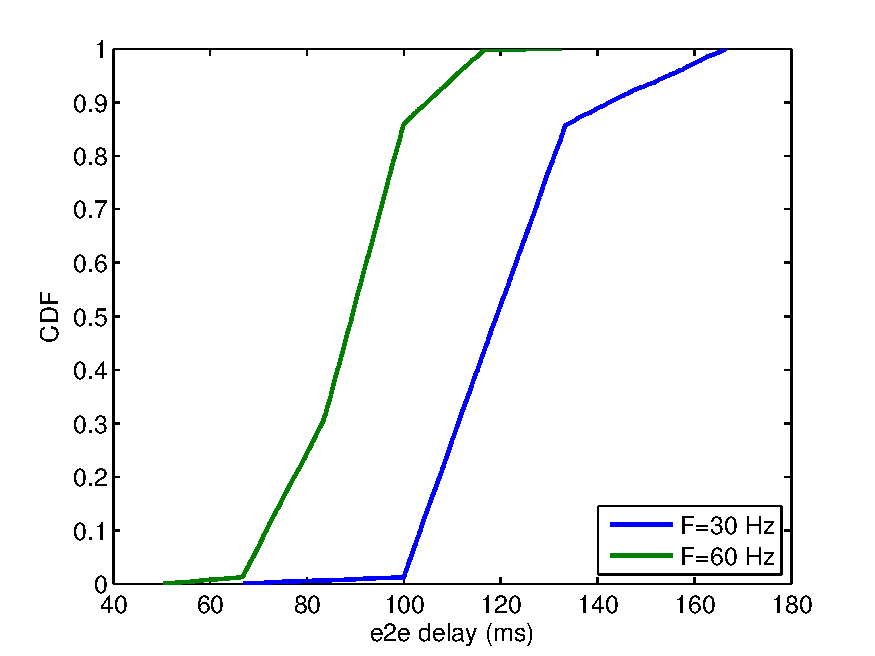
\includegraphics[width=1.0\columnwidth]{images/e2e-delay-sim.pdf}
% 	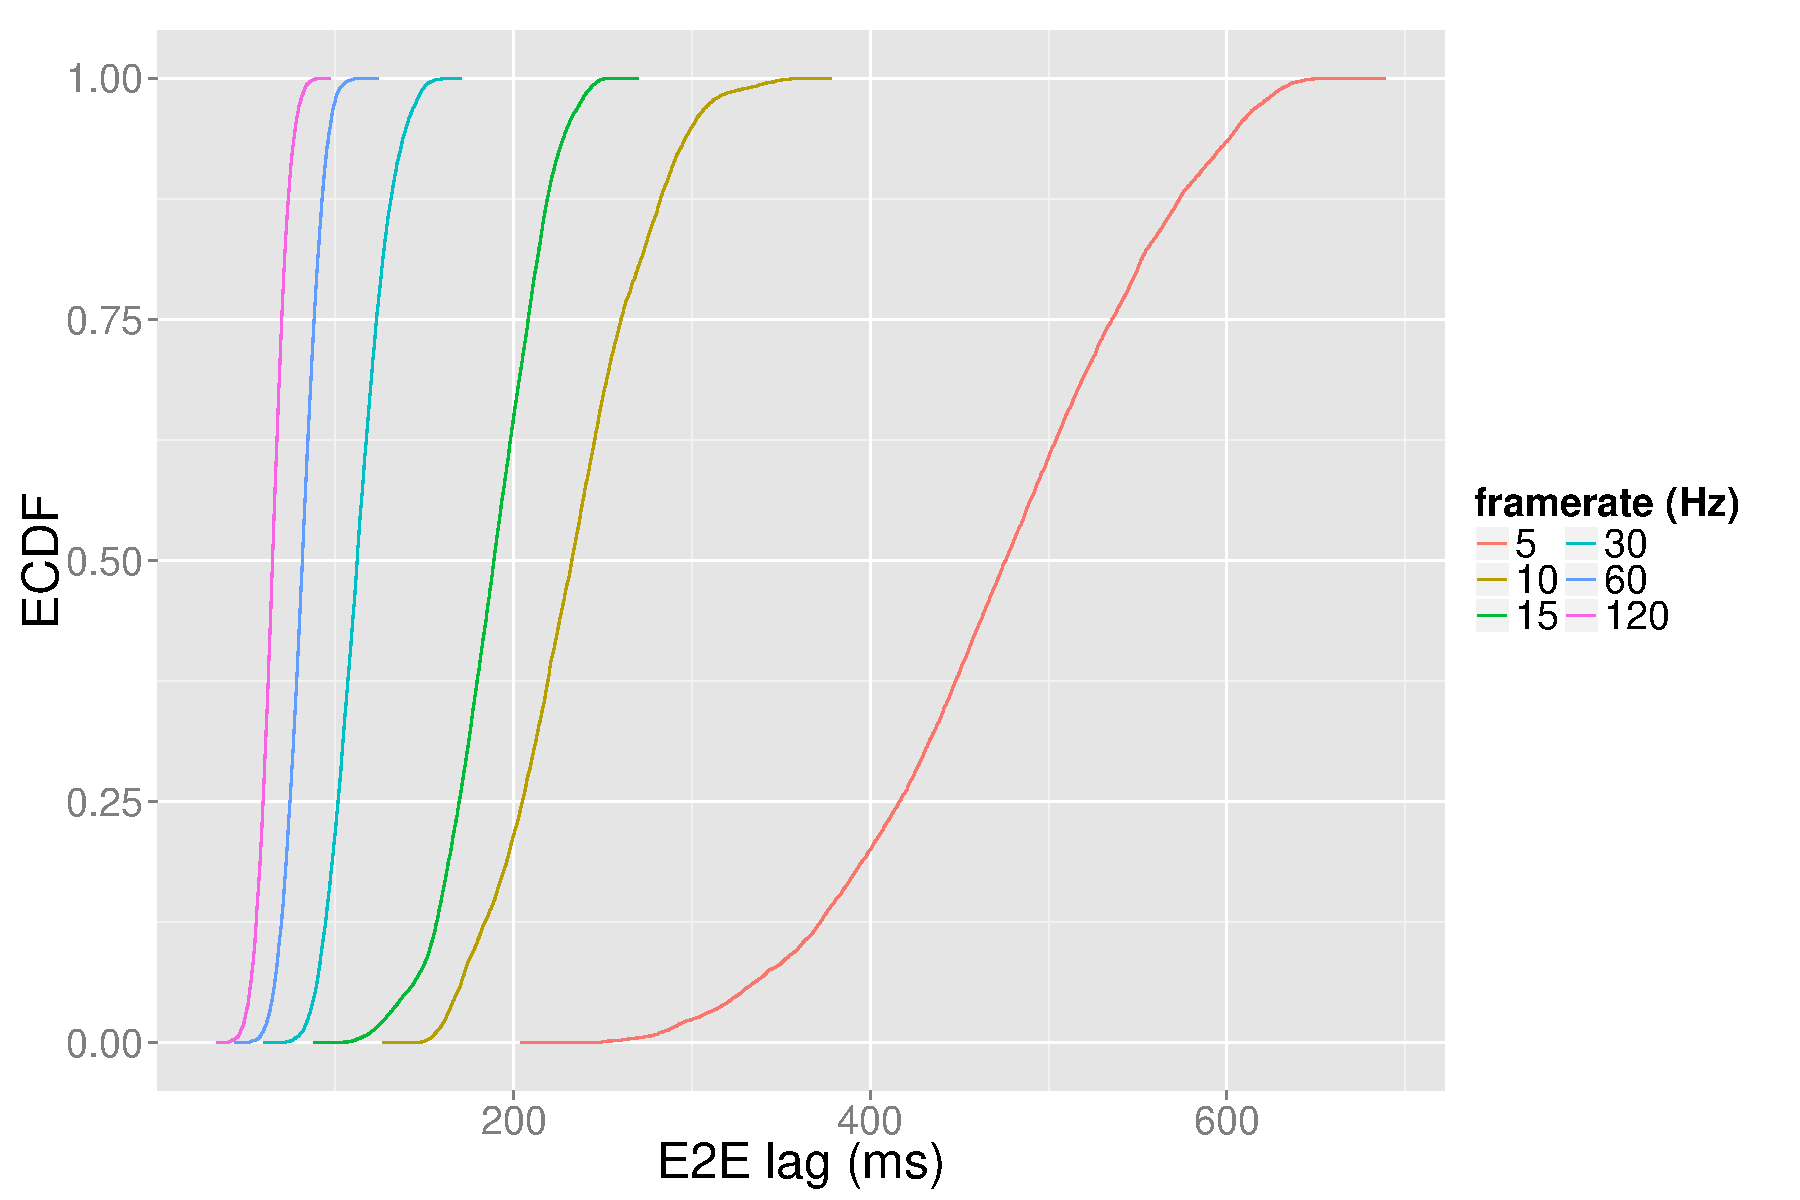
\includegraphics[width=1.0\columnwidth]{../../simulation/visualization/cloudgaming-lag-cdf.pdf}
% 	\caption{\acrshort{ECDF} of the influence of the rendering and streaming framerate on the end-to-end lag in the cloud scenario. Vertical intercept denotes the average base delay of $\SI{68}{\milli\second}=c^{-1}+2D+P+e+d$.}
% 	%\hoss{On average, a network delay of $\unit[2\cdot20=40]{ms}$ (correct???) exists. A constant encoding time (\unit[15]{ms}) and decoding time (\unit[5]{ms}) is assumed. Thus, the major part of the e2e lag is caused by the framerate setting. Kann man hier noch eine Linie reinzeichnen, die die Summe 5+15+40=60 ms zeigt?}}
% 	%
% 	% Albert: Uh, oh, the cloud simulation seems to have reused a stray 
% 	%         200 Hz setting for $c$ from a previous online game sim.
% 	%         I'm documenting that this value has been used.
% 	%
% \label{fig:cloud-e2e-delay-sim}
% \end{figure}

% Figure~\ref{fig:cloud-e2e-delay-sim} shows the results of this scenario as an \gls{ECDF} of the end-to-end lag for several framerates. As before, the framerate impacts the end-to-end lag more severely than the network delay.
% %the large influence of the framerate when compared to the network delay is evident. 
% This result is of particular importance considering how past studies have relied on similarly low framerates as $5-\SI{15}{\hertz}$ when assessing the network influence on cloud gaming. Similarly, these results can provide guidelines for implementors of cloud gaming to factor in the framerate in their calculations accordingly.


%%%%%%%%%%%%%%%%%%%%%%%%%%%%%%%%%%%%%%%%%%%%%%%%%%%%%%%%%%%%%%%%%%%%%%%%%%%%%%%%
% \subsubsection{Discussion}




%%%%%%%%%%%%%%%%%%%%%%%%%%%%%%%%%%%%%%%%%%%%%%%%%%%%%%%%%%%%%%%%%%%%%%%%%%%%%%%%
%\subsection{Reasonable Configuration/Setting Ranges to Test}

% Resolution: Minimum 720p, 1080p recommended, even higher is better (1440p or 2160p)
% Frame rate: 60 fps very much recommended, 30 absolute minimum,  120 or 144 can also be feasible
% Configure games to run at high or at least medium settings
% For console games: use the games intended settings for the console, never downscale the game or reduce the frame rate for streaming
% Assume no network latency higher than 200ms, preferably less than 100ms
% Assume typical access link conditions, i.e. no less than 10-16Mb/s



%Works only for general purpose computing devices with full access.
%Easiest method, but might not capture full end-to-end latency.
%FRAPS, OBS, DirectX Hooking, MSI Afterburner
%FCAT as hybrid solution with external capture card and computer


% \url{http://www.red.com/learn/red-101/high-frame-rate-video}


% articles:
% why frametimes
%     \url{https://techreport.com/review/21516/inside-the-second-a-new-look-at-game-benchmarking}

% Inside the second with Nvidia's frame capture tools
%     \url{https://techreport.com/review/24553/inside-the-second-with-nvidia-frame-capture-tools}

 % As the second turns: the web digests our game testing methods
 %    \url{https://techreport.com/blog/24133/as-the-second-turns-the-web-digests-our-game-testing-methods}

% GPU Reviews: Why Frame Time Analysis is important
%     \url{http://www.vortez.net/articles_pages/frame_time_analysis.html}

% Durante's Witcher 3 analysis: the alchemy of smoothness
%     \url{http://www.pcgamer.com//durantes-witcher-3-analysis-the-alchemy-of-smoothness/}


% Analysing Stutter – Mining More from Percentiles
%     \url{https://developer.nvidia.com/content/analysing-stutter-%E2%80%93-mining-more-percentiles-0}

% fraps vs fcat method
%     \url{http://www.extremetech.com/gaming/154089-after-almost-20-years-gpu-benchmarking-is-moving-past-frames-per-second}

% FRAPS + FRAFS
% \url{http://www.fraps.com/}
% \url{http://sourceforge.net/projects/frafsbenchview/}
% \url{http://www.5group.com/wordpress/2012/07/14/gpu-mist-pre-release-1-0-rc1/}

% issue: Fraps measures the flip queue input rather then the actual render output frames which is fine when measuring FPS but is rather poor if you want to measures actual frame times and analyze microstutter.


% NVIDIA FCAT
% \url{http://www.geforce.com/hardware/technology/fcat}
% \url{http://www.overclockers.com/nvidias-fcat-gpu-testing-pursuing/}


% Valve for Linux GL Games
% \url{https://github.com/ValveSoftware/voglperf}

% Info über MSI Afterburner overlay? oder GF experience? GPU-Z? Rivatuner Statistics Server?
% \url{http://www.overclock.net/a/how-to-use-rivatuner-afterburner-on-screen-display-and-more}



% \url{https://en.wikipedia.org/wiki/Game_classification}
% \url{https://en.wikipedia.org/wiki/Video_game_genre}
% \url{https://en.wikipedia.org/wiki/List_of_video_game_genres}








%%%%%%%%%%%%%%%%%%%%%%%%%%%%%%%%%%%%%%%%%%%%%%%%%%%%%%%%%%%%%%%%%%%%%%%%%%%%%%%%
% \subsection{Sources of Latency in Gaming}
% \label{sec:latency}






%All in all, if possible, video game measurements should always consider the full \textbf{end-to-end} lag factoring in every possible source of delay but also the presence latency compensation and concealment techniques.



% Online games attempt to compensate network latency through various means, such as already showing the results of your local inputs while waiting for the authoritative update from the server and potentially rolling back the local updates.

% TODO: Also mention lag compensation/concealment techniques:
% Client-side: non-authoritatively update game state based on own inputs and merging it afterwards with the server's view, correcting any prediction errors
% Server-side: Keep a short history of past game states, and do not execute player commands at the state they were received but rather at the (estimated) state time they were intended for.

% lag compensation can also be implemtented specifically for cloud gaming as the work conducted in \cite{Lee:2015:OUS:2742647.2742656} suggests, however incurring siginficant overhead in terms of processing time for the game logic and renderer as well as the encoding and bandwidth due to specutatively generating and transmitting frames ahead of their corresponding input.


% game keeps history of recent game state snapshots to interpolate between two server states and create a smoother experience (thus decoupling client frame rate from the server's state updates), but adds e.g. \SI{100}{\milli\second} of view lag due to snapshot history.


%%
%\subsubsection{Online Video Game Latency Concealment Techniques}


% input: absolute (eg mouse) vs. relative (analog stick)
% frame perfect input
% double/triple buffering
% inputs per minute vs timing precision of input
% range of interactivity
% latency sensitivity/responsiveness of different game mechanics / UI elements in the same game
% latency of camera movement / UI vs actual game elements


%Info on source engine networking: \url{https://developer.valvesoftware.com/wiki/Source_Multiplayer_Networking}
%\url{https://developer.valvesoftware.com/wiki/Latency_Compensating_Methods_in_Client/Server_In-game_Protocol_Design_and_Optimization}
%(Latency Compensating Methods in Client/Server In-game Protocol Design and Optimization, Yahn W. Bernier (yahn@valvesoftware.com), 2001, Software Development Engineer, Valve Software)



% Online games generally follow one of two designs. Either there is a dedicated server available to host the game, or one of the clients is elected to additionally act as the server.
% The election is typically based on criteria such as the available performance and latency. If the selected host drops out of the game, a new server has to be elected and the game gets migrated there, usually stopping the game for a few moments. Competitive games almost always choose the dedicated approach to ensure fairness, stability and better control cheats.



% \begin{figure*}[!t]
% 	\centering
% 	\begin{subfigure}[b]{0.5\textwidth}
% 		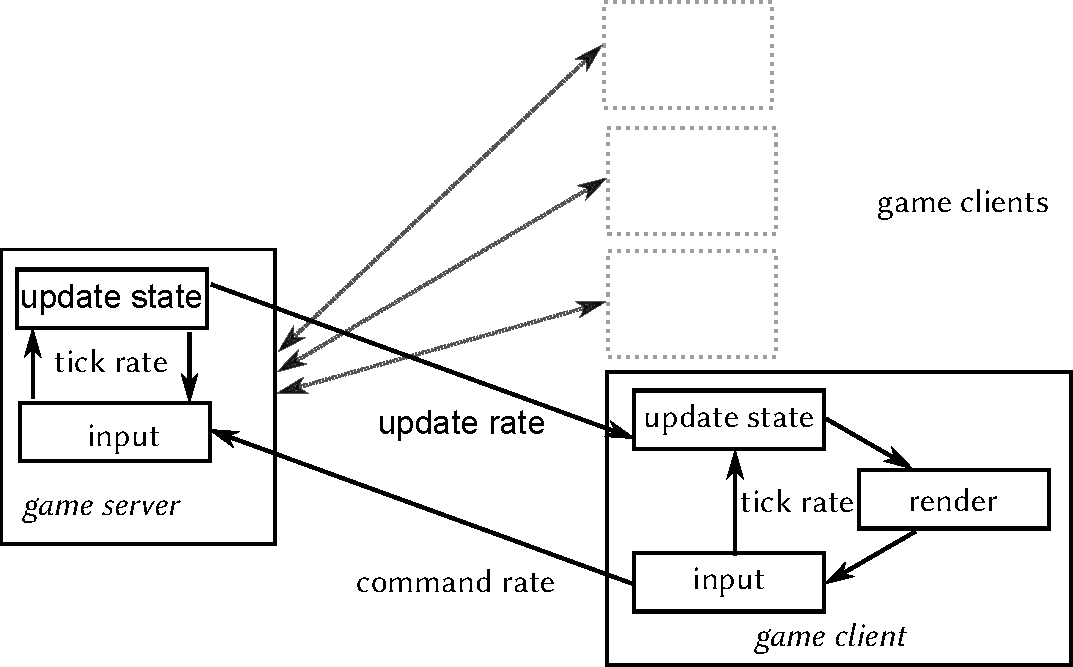
\includegraphics[width=1.0\columnwidth]{images/game-tick-rate.pdf}
% 		\caption{In typical online games.}
% 		\label{fig:tickrate-online}
% 	\end{subfigure}%
% 	~
% 	\begin{subfigure}[b]{0.5\textwidth}
% 		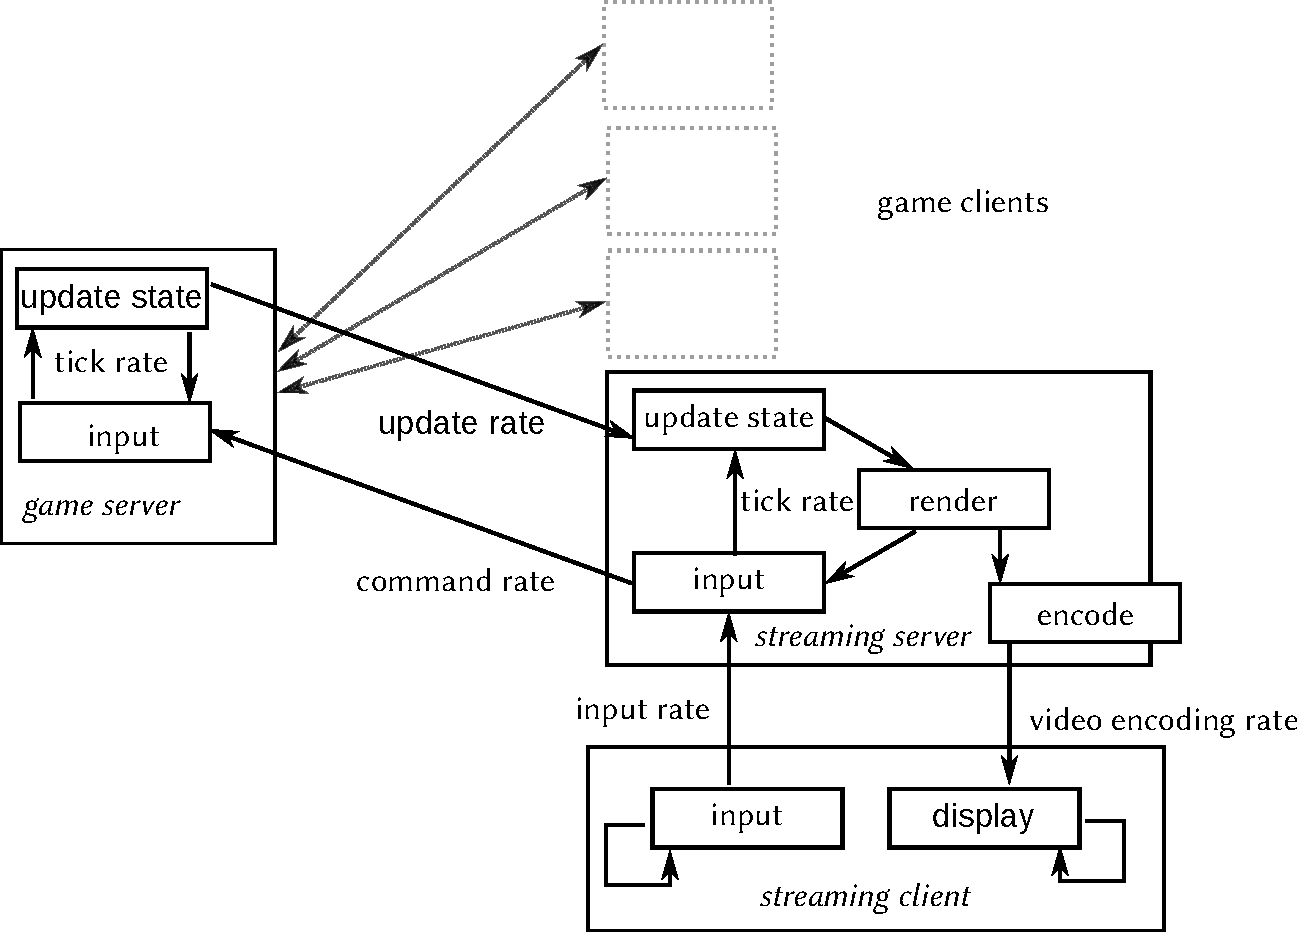
\includegraphics[width=1.0\columnwidth]{images/game-tick-rate-streamed.pdf}
% 		\caption{In a cloud gaming scenario.}
% 		\label{fig:tickrate-streamed}
% 	\end{subfigure}
% 	\caption{Interaction of the game client and server.}
% 	\label{fig:tickrates}
% \end{figure*}



% \begin{figure}[!t]
% 	\centering
% 	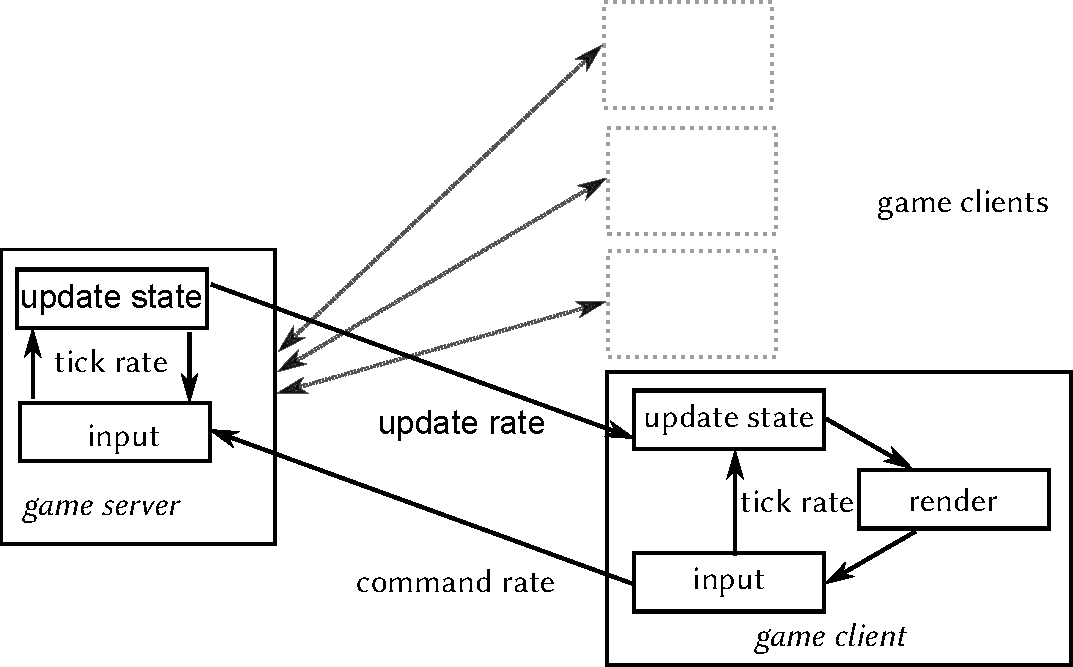
\includegraphics[width=1.0\columnwidth]{images/game-tick-rate.pdf}
% 	\caption{Interaction of client and server in typical online games.}
% \label{fig:tickrate-online}
% \end{figure}








% \subsection{Determining Video Game Popularity and Engagement}
% FUTURE WORK!

% Using Steam data as a popularity measure and get a grasp of which games could be worthwhile to look at. Ties in to user engagement metrics to determine the quality a game delivers in a current situation. Alternative view: the more engaged players are to a game, the more important is delivering a good quality (e.g. for streaming).

% For example, there might be a correlation between a game's price and the average time it's been played, as Figure~\ref{fig:tickrate-streamed}.


% Other  k-means clustering of steam/price data or other graphs

% \begin{figure}[!t]
% 	\centering
% 	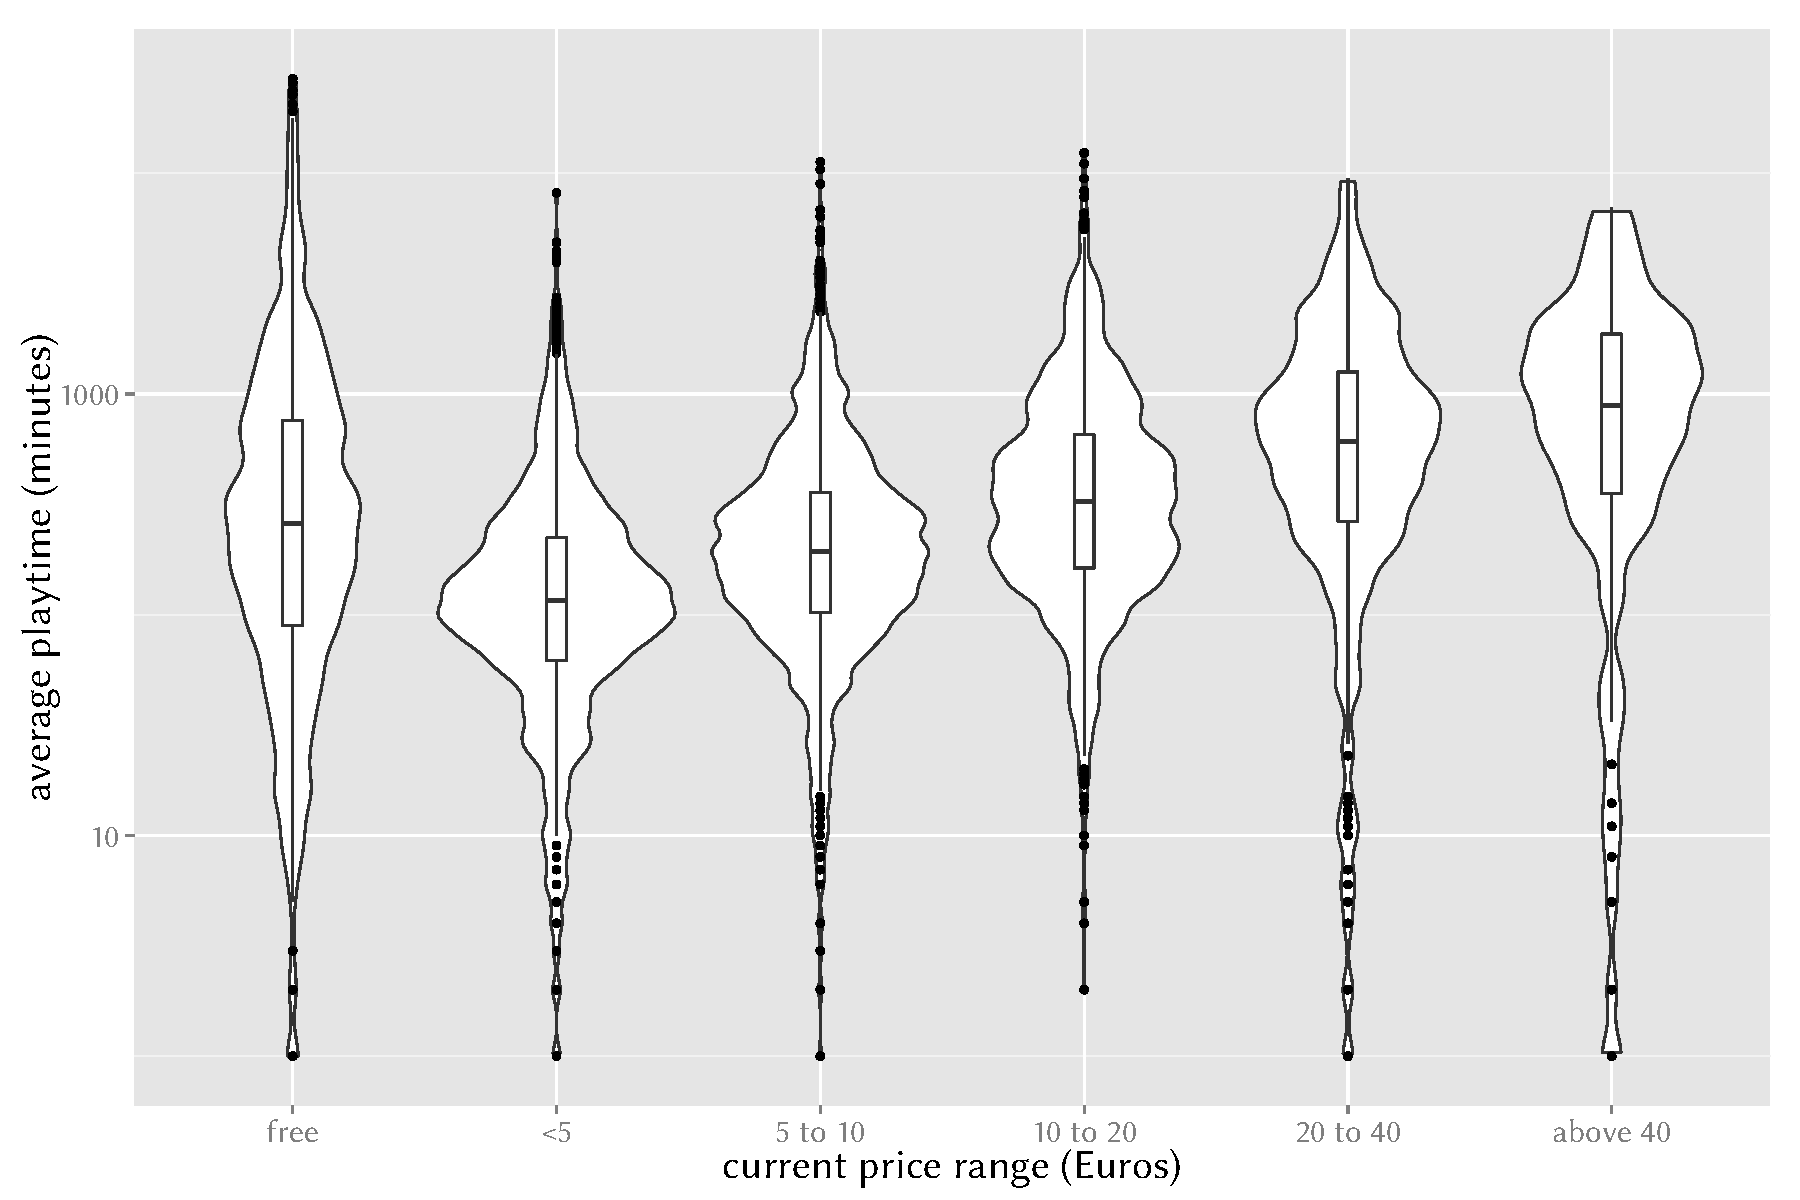
\includegraphics[width=1.0\columnwidth]{images/dampfviolinen-playtime.pdf}
% 	\caption{Game cost as a possible categorization and engagement factor. Displayed is a violin plot of the current costs in relation to the average playtime of individual games.s}
% \label{fig:cost-playtime-violin}
% \end{figure}

% Categorization dimensions viable for measuring online video game quality:



%\footnote{\url{http://accidentalscientist.com/2014/12/why-movies-look-weird-at-48fps-and-games-are-better-at-60fps-and-the-uncanny-valley.html}}
%\url{https://stackoverflow.com/questions/17411/how-do-you-separate-game-logic-from-display}
%\url{http://higherorderfun.com/blog/2010/08/17/understanding-the-game-main-loop/}
